\chapter{Task}

A problem of classification or regression had to be selected, that could be solved with means of Machine learning. For the solution there were two approaches possible; the classical ML approach and the deep learning approach. For the chosen problem, the right approach had to be used and implemented. The topology and structure of the implementation had to be explained. After creating a model, it had to be evaluated and tested by at least two different model evaluation metrics. Finally a conclusion had to be drawn about the model in relation to the problem. The task description was available on \href{https://moodle.htw-berlin.de/mod/assign/view.php?id=413684}{Moodle}.

\chapter{Problem}

I chose to do the deep learning approach. I used the website kaggle.com to look for a dataset containing a larger amount of images to be able to classify them with a computational neural network (CNN). 

The dataset i selected was "Flowers Recognition"  and contains in total 4242 images of five different types of flowers.\footnote{\label{foot:1}\href{https://www.kaggle.com/alxmamaev/flowers-recognition/home}{https://www.kaggle.com/alxmamaev/flowers-recognition/home}}. The images were scraped from different image sources online like Google Image, flickr etc. Because of that, they are in different sizes and resolutions and need to preprocessed before feeding them into a CNN. 

Because of the large amount of available data, the deep learning approach was ideal for this type of problem.

\chapter{Implementation}

The code structure was taken from the one on moodle\footnote{\label{foot:2}\href{https://moodle.htw-berlin.de/mod/resource/view.php?id=417224}{https://moodle.htw-berlin.de/mod/resource/view.php?id=417224}} and consists of two python code files. (inside the directory \texttt{code/}) 

\texttt{code/my\_cnn\_train.py} includes the training of the convnet and basic loading function for reading and preparing the dataset. The created model is saved at the end as \texttt{mymodel.dat} and can be used to directly classify images without having to train the model first. 

In \texttt{code/my\_cnn\_test.py}, the model that was created and saved in the previous file, is read by \pyth{keras} and used to classify some images. The results are shown with \texttt{openCV}, where every given image is printed with the most likely result label. (Again, this was mostly taken from the sample code on moodle)

The dataset is inside the directory \texttt{flowers}. It contains five subdirectories, one for each label / flower type. Each of those directories contains about 800 images in \texttt{JPG} format. The exact amount can be found in table \ref{tab:flower_distrib}.

\begin{table}[h]
	\centering
	\begin{tabular}{|c|c|@{}} 
		\hline
		\textbf{type}& \textbf{number of images}	
		\\ \hline
		daisy	& 765
		\\ \hline
		dandelion	& 1095		
		\\ \hline
		rose	& 784	
				\\ \hline
		sunflower	& 734
				\\ \hline
		tulip	& 984		
		\\ \hline
		
	\end{tabular}
	\captionof{table}[distribution of flower types]{\textbf{distribution of flower types}}
	\label{tab:flower_distrib}
\end{table}

Detailed explanation of code is found in the source files as comments.

Everything was implemented and tested on Windows 10 (64 bit) with Visual Code.

\section{training}

The function \pyth{create_model()} is responsible for building the different layers of the model and returning the final model at the end.
\inputpython{code/my_cnn_trainLATEX_NICHT_ABGEBEN.py}{3}{10}

To read the image data, a second function \pyth{load_dataset()} was used.
\inputpython{code/my_cnn_trainLATEX_NICHT_ABGEBEN.py}{3}{10}

\section{testing}

\inputpython{code/my_cnn_testLATEX_NICHT_ABGEBEN.py}{3}{10}


\chapter{Evaluation}

To evaluate the created model, multiple metrics were used:

\begin{itemize}
	\item accuracy
	\item Precision / recall
	\item AUC-ROC
	\item f1 score
\end{itemize}

\section{accuracy}
Accuracy is the simplest metric because its just right divied by wrong. I achieved a maximum accuracy of around XX percent.

\section{precision/recall}
precision and recall can be calculated as formeln hier
The precision / recall curve can be seen in figure \ref{chart:prec_rec_curve}.

\begin{figure}
	\centering
	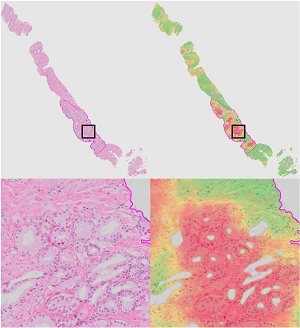
\includegraphics[scale=0.5]{images/CHANGE_THIS.png}
	\caption{precision / recall curve}
	\label{chart:prec_rec_curve}
\end{figure}

\section{AUC-ROC}
AUC-ROC is an abbreviation for blabla.
The AUC\_ROC is shown in figure \ref{chart:auc_roc}.

\begin{figure}
	\centering
	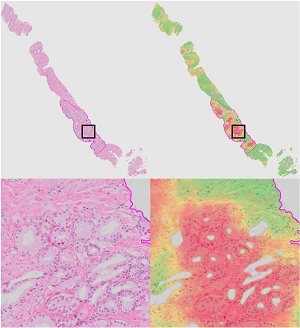
\includegraphics[scale=0.5]{images/CHANGE_THIS.png}
	\caption{AUC\_ROC}
	\label{chart:auc_roc}
\end{figure}

\section{f1 score}
The F1 score is displayed in figure \ref{chart:f1_score}.

\begin{figure}
	\centering
	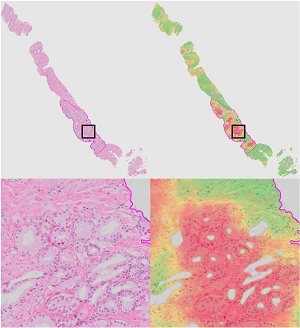
\includegraphics[scale=0.5]{images/CHANGE_THIS.png}
	\caption{F1 score}
	\label{chart:f1_score}
\end{figure}

\chapter{Conclusion}

Using an image dataset of over 4000 images of flowers, a conv net was build and used to classify new images of flowers. The model achieved an accuracy of XX percent, as described in the last chapter. 

Does the selected model fit the result? Yes because conv net is good for images, esp for many.
Influeing paremters: Using dropout to make it indepent more and not prone to overfitting.
Epochs: traing longer takes more time, wird es besser wenn man viel mehr nimmt?